\subsection{Conductivity}
As mentioned in the Design Report, the DFRobot DFR0300H \cite{DFR0300H} was chosen for measuring the conductivity. The manufacturer claims the sensor has an accuracy of 5\% FS, meaning with a range of 20ms/cm, it has an error of 1ms/cm. 

\begin{table}[h!]
	\centering
	\adjustimage{height=4cm,valign=c}{sensors/23_dfr0300h.jpg}\quad
	\begin{tabular}{| l | l |}
    \hline
    Protocol & Analog\\
    Measurement Accuracy &  5\% FSR\\
    Supply Voltage & 3.3-5V\\
    Support Detection Range & 10~100ms/cm\\
    Software library included & yes \\
    Probe included & yes \\
    Availability & 3-5 Working days \\
    \hline
	\end{tabular}
\end{table}

\subsubsection{Known conductivity solutions}
Known conductivity solutions of 12.88ms/cm and 1.413ms/cm were used to determine the accuracy of the sensor.

\begin{figure}[h]
  \centering
  \begin{minipage}[b]{0.7\textwidth}
    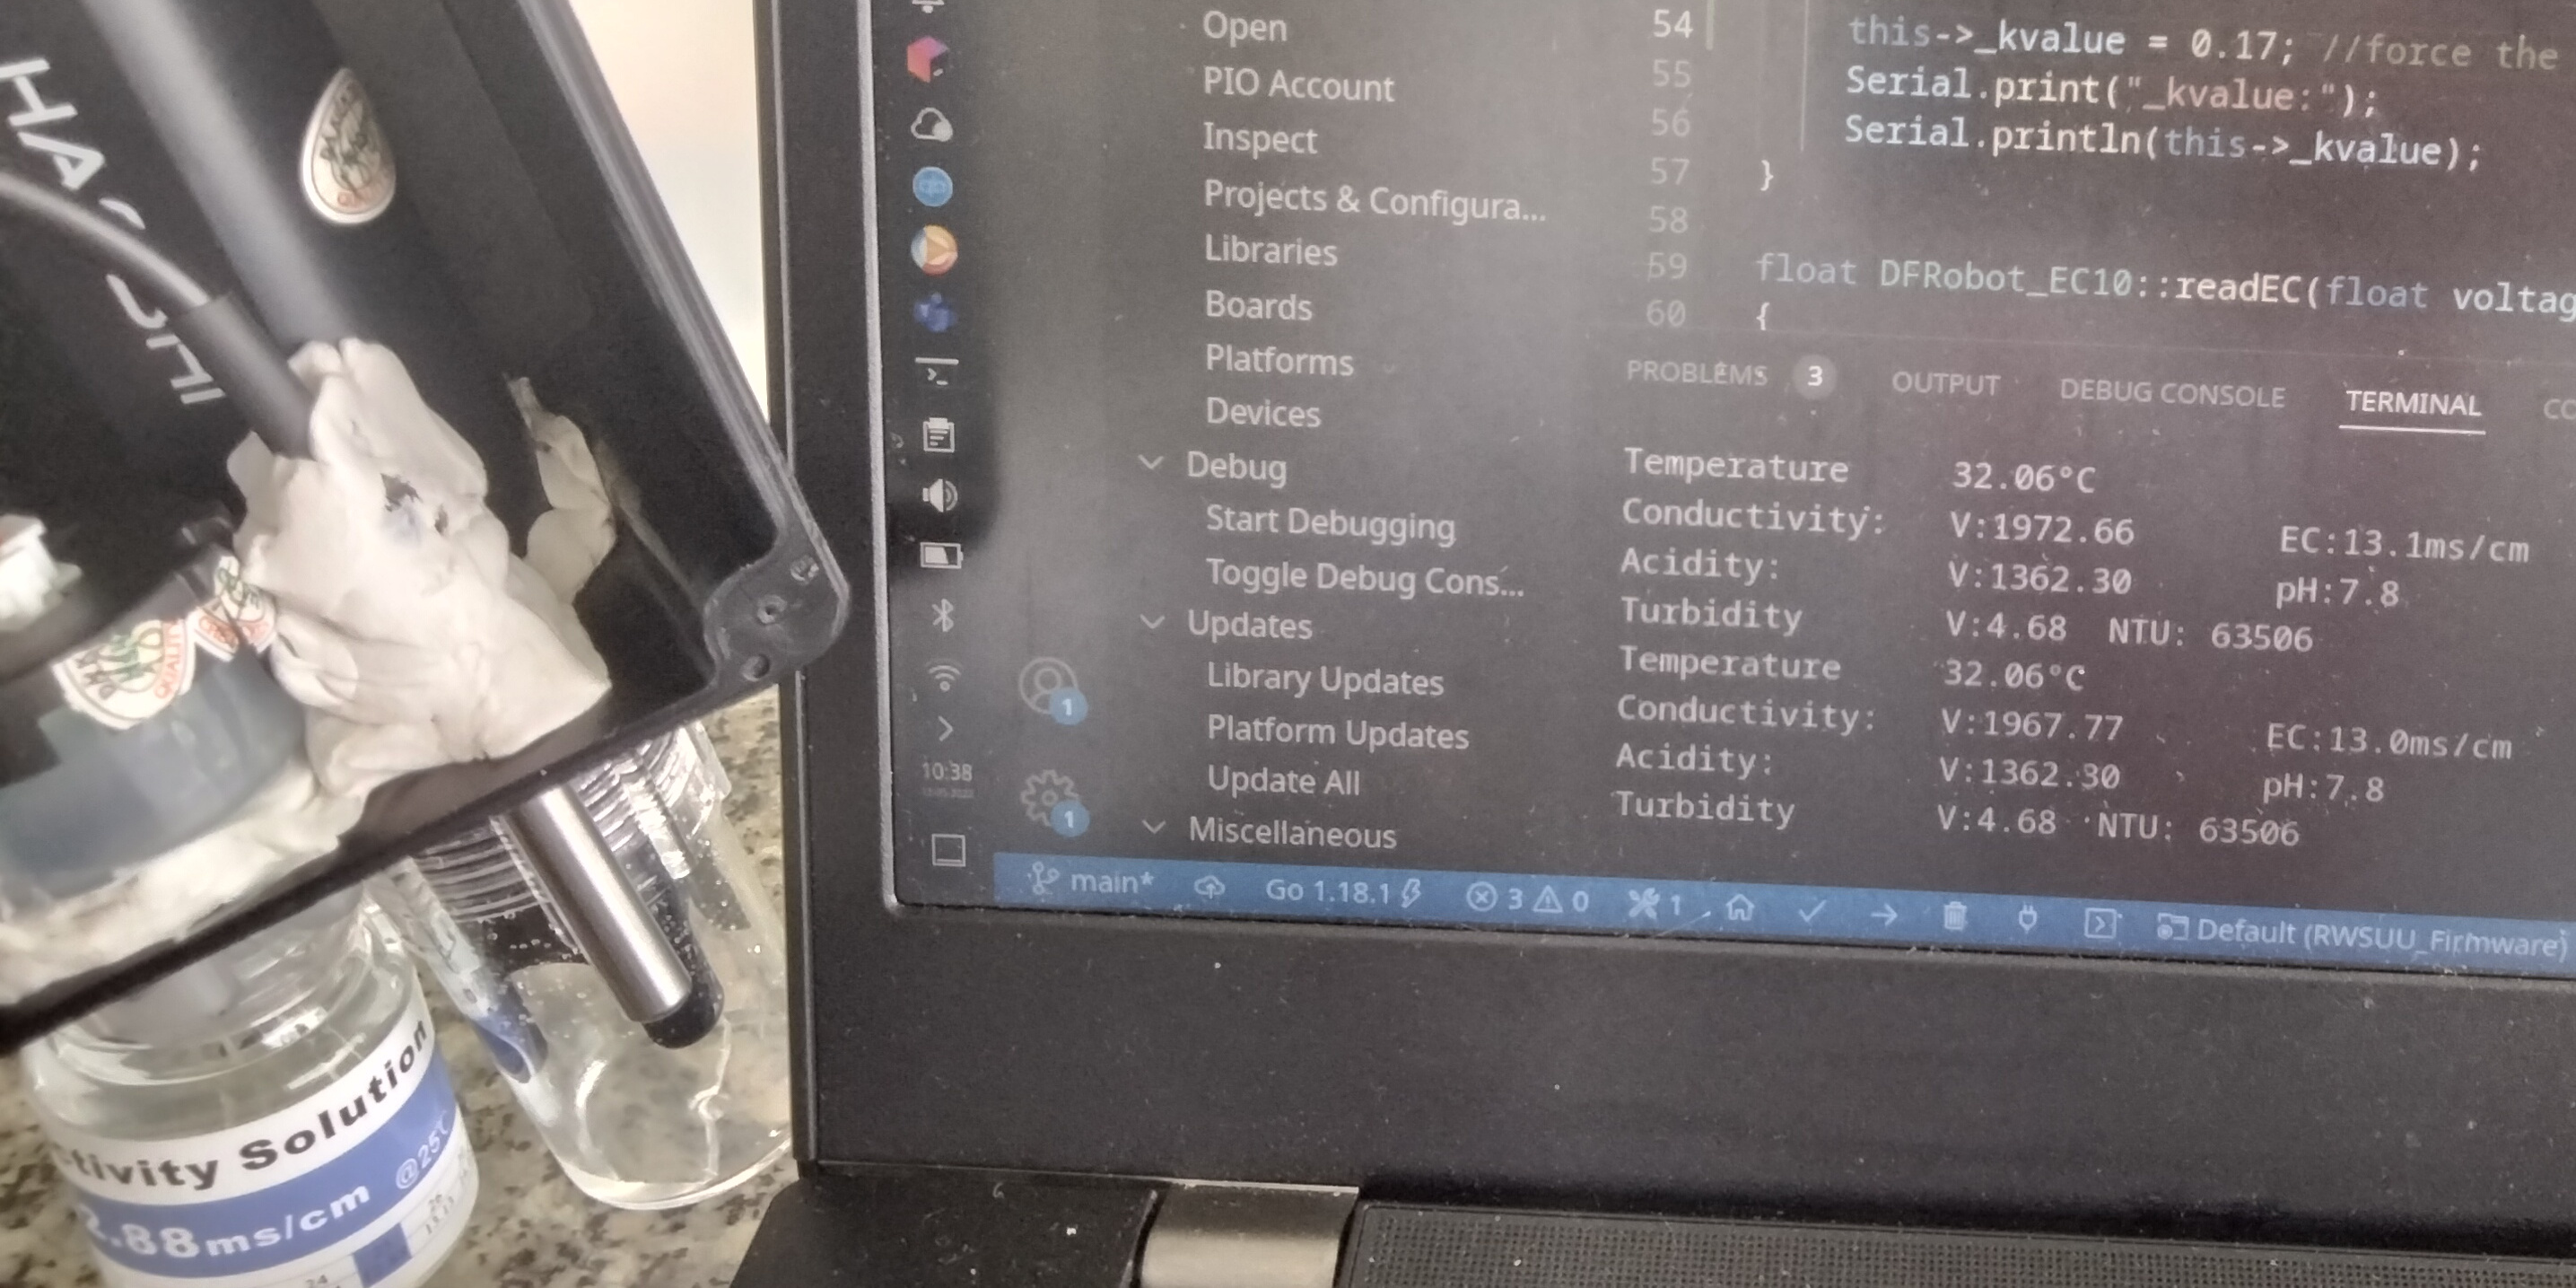
\includegraphics[width=\textwidth]{sensors/21_ec1288_dfrobot.jpg}
    \caption{measured 13.0 at 12.88ms/cm solution}
  \end{minipage}
  \hfill
  \begin{minipage}[b]{0.7\textwidth}
    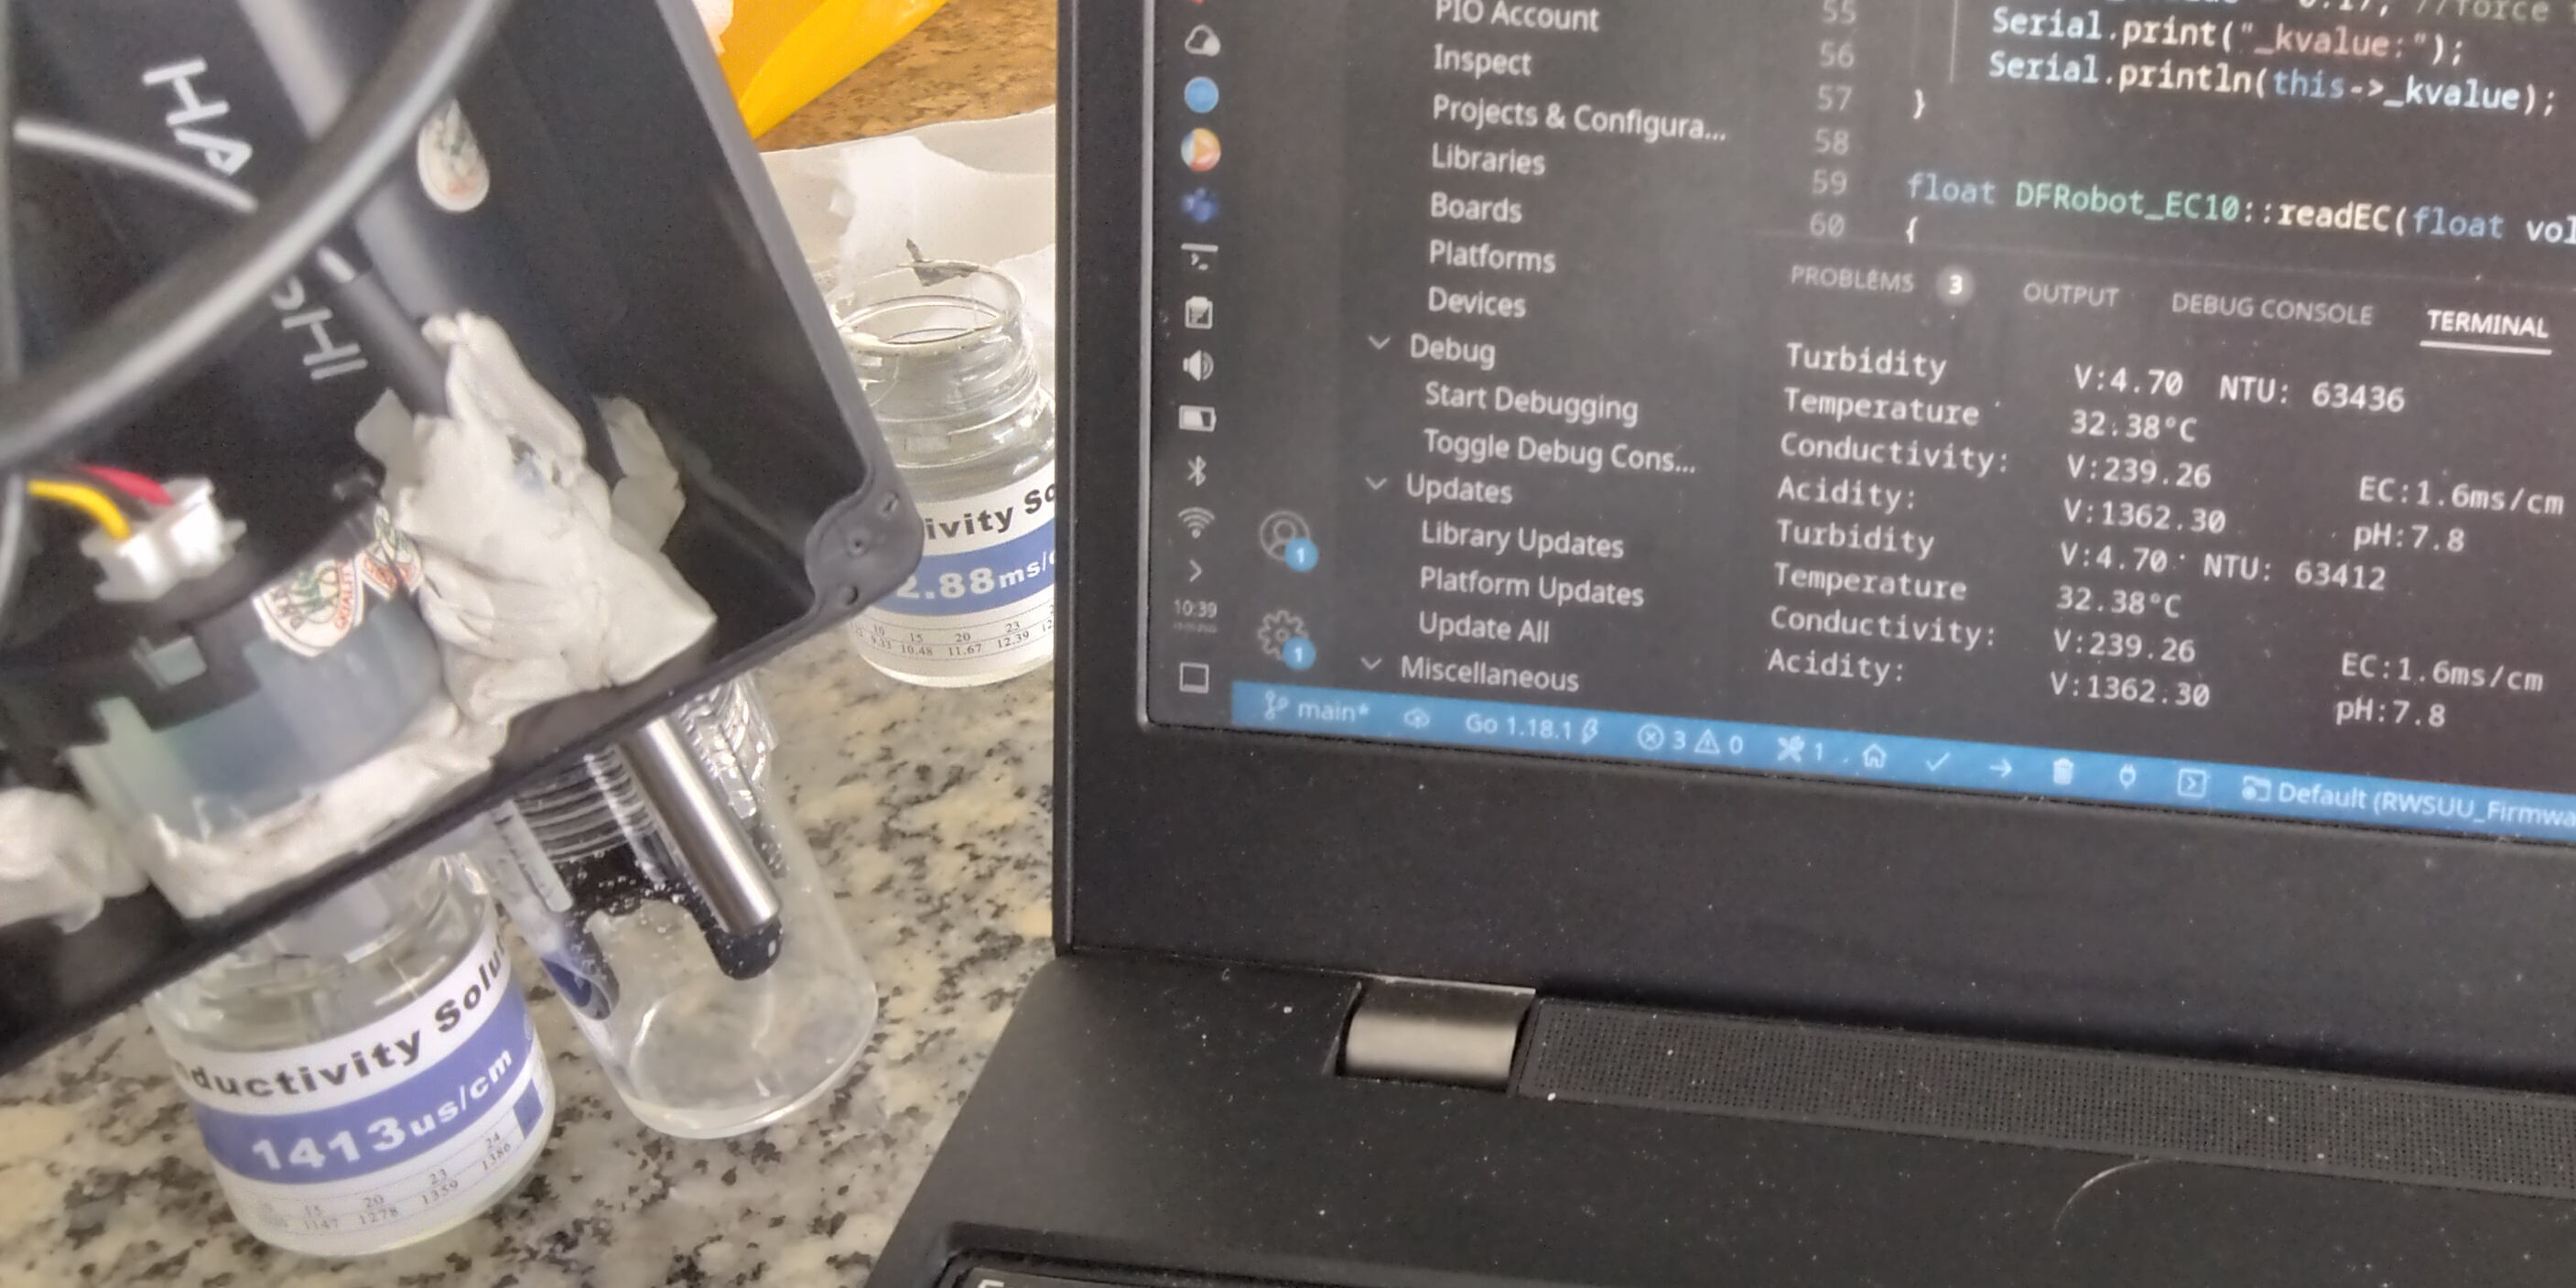
\includegraphics[width=\textwidth]{sensors/22_ec1413_dfrobot.jpg}
    \caption{measured 1.6 at 1.413ms/cm solution}
  \end{minipage}
\end{figure}